\documentclass[11pt]{article}
\usepackage[utf8]{inputenc}
\usepackage[T1]{fontenc}
\usepackage[brazil, english]{babel}
\usepackage{amsmath}
\usepackage{amsfonts}
\usepackage{graphicx}
\usepackage{setspace}
\usepackage{geometry}
\usepackage{indentfirst}
\usepackage[small,bf]{caption}

\begin{document}
\selectlanguage{brazil}
\begin{titlepage}
\begin{center}
\textsc{\Large Resumo e Cronograma Detalhado do Projeto\\}
%\textsc{\small Fundação de Amparo à Pesquisa do Estado de São Paulo - FAPESP}\\[6.5cm]
% \textsc{\Huge Quebra de simetria espontânea, Limites Cognitivos e  Complexidade de Sociedades}\\[0.5cm]
\textsc{\small {\it Estudante:} felippe alves pererira\\ {\it Orientador:}
nestor caticha\\}
% \vfill
\textsc{universidade de são paulo - instituto de física}\\
\textsc{\small departamento de física geral}\\
\small \today
\end{center}
\end{titlepage}

\newpage

\selectlanguage{brazil}
% \doublespace

\newpage\null\thispagestyle{empty}\newpage
\section{Resumo}

Remontam aos primórdios do pensamento humano as questões sobre sua própria
natureza, em várias de suas manifestações. Dentre elas, aquelas sobre
o surgimento das sociedades e outras instituições de caráter cooperativo como
produto das interações entre pessoas têm sido objeto de estudo 
nos últimos anos e têm mostrado resultados interessantes
\cite{CatichaetalA,Schonmannetal2011a,Perreault,Jonatas,visujeca}. 

É dentro desse contexto que este projeto está inserido. Mais especificamente, o
objetivo do projeto é buscar novas perguntas e novo conhecimento sobre o
surgimento, estabilidade e coexistência de grupos com diferentes valores morais
e aplicar esse conhecimento no entendimento
da origem de crenças, pensamento religioso, ou instituições religiosas.

Para esse fim, é preciso formular perguntas, e modelos para responder estas
perguntas, que possibilitam verificar a existência de uma
instituição, grupo ou organização, a partir da interação entre indivíduos ao
longo do tempo. É necessário também entender o mecanismo de interação e
sua relação com cada indivíduo. A seguir, uma abordagem mais detalhada da
estratégia usada neste projeto para atacar o problema proposto.

\subsection{Teoria dos Fundamentos Morais e Modelos de Agentes}

A Teoria dos Fundamentos Morais, proposta pelo psicólogo social {\it J.
Haidt} \cite{Haidt}, traz duas características importantes para a compreensão
da moralidade humana. A primeira é que os julgamentos morais ocorrem de forma
espontânea e (para todos os efeitos imediata) quando uma pessoa é exposta a uma
questão de cunho moral. Isso significa que não há tempo para o raciocínio
interfirir na consequência dessa exposição, ou que toda racionalização 
acontece após tal consequência. A segunda diz respeito a caracterização das
bases morais. Segundo {\it Haidt}, ao menos $5$ bases morais são relevantes,
sendo elas:
\begin{enumerate}
    \item Violência / Cuidado
    \item Justiça / Trapaça
    \item Lealdade ao grupo / Traição
    \item Respeito à autoridade / Subversão
    \item Santidade (ou Pureza) / Degradação
\end{enumerate}

Essas duas características são importantes pois possibilitam a elaboração de
modelos de agentes caracterizados por um vetor em $5$ dimensões 
que determina
sua matriz moral, nos quais é possível estabelecer uma interação instantânea. 
Isso permite que os agentes possam viver
uma dinâmica onde suas opiniões dependem de um aprendizado prévio (ou em curso)
e que permita a emergência de coletividade no campo das opiniões.

\subsection{O modelo básico proposto}

No espírito de formular perguntas em cima da plataforma estabelecida pela Teoria
dos Fundamentos Morais e da ideia de modelos de agentes, é proposto um modelo
básico, do qual variações simples permitem o teste de diferentes hipóteses. Esse
modelo deve capturar as características destacadas acima e permitir o uso de
técnicas bem estabelecidas, como os métodos da mecânica estatística e teoria do
aprendizado de máquina. 

Considere um sistema formado por $N$ agentes, sendo cada um deles caracterizado
por um vetor $w_i \in \mathbb{R}^D$, com $i \in \{1,\ldots,N\} = V$ e $|w_i|=1$ 
para
todo $i$. 
Os vetores $w_i$ representam a matriz moral de cada agente, na qual reside as
bases de suas opiniões (definidas adiante).

Esses agentes estão dispostos numa rede social de interações
caracterizada pelo grafo $\mathcal{G}=(V,E)$, onde $V = \{1,\ldots,N\}$,
conjunto
dos índices dos agentes, são os vértices e $E$ as arestas do grafo, do qual um
elemento é denotado por $(ij)$ quando os agentes $i$ e $j$ 
interagem (são primeiros vizinhos no grafo).

Sejam, também, $x^{\mu} \in
\mathbb{R}^D$, com $\mu \in \{1,\ldots,P\}$ e $|x^{\mu}|=1$ para todo $\mu$, um
conjunto de questões morais às quais os agentes serão expostos. 
A opinião de um agente $i$ sobre uma questão $\mu$ é definida pelo produto
escalar dos vetores $h_i^{\mu}=w_i \cdot x^{\mu}$. O lado ou a postura desse
agente com relação a essa questão é dada pelo sinal da opinião
$\sigma_i^{\mu}=\mathrm{sgn}(h_i^{\mu})$.

Essa base permite o uso dos resultados da teoria de aprendizado supervisionado
para uma rede neural de uma camada. Tal
situação demanda uma rede aluno e uma rede professor e mostra que, dado um
número suficientemente grande de exmplos, caso as redes aluno e professor tenham
a
mesma dimensão, então a rede aluno consegue imitar a rede professor. Cada
exemplo é composto por um vetor questão e uma resposta dada pelo sinal do
produto escalar do vetor professor com o vetor questão.
Além disso, é possível mostrar \cite{Engel} que essa dinâmica de
aprendizado pode ser vista como a descida pelo gradiente de um potencial de
interação entre aluno e professor.

Seguindo o modelo proposto em \cite{visujeca}, considere o cenário em que
um par de agentes, $(ij)$ interage através da troca de opiniões a respeito de uma
questão moral. Digamos que, no instante $t$, o agente $i$ é o aluno e $j$ o
professor, de modo que o exemplo recebido por $i$ é $(x^{\mu}, \sigma_j^{\mu})$.
Então o agente $i$ atualiza sua matriz moral da seguinte forma:

\begin{equation*}
    w_i(t+1)= w_i(t)+\eta x^{\mu}\nabla_{w_j}V_{\delta}(h_i^{\mu}h_ j^{\mu})
\end{equation*}

com o potencial de interação entre agentes dado por

\begin{equation}
    V_{\delta}(h_i^{\mu}h_j^{\mu})=-\frac{1+\delta}{2}h_i^{\mu}h_j^{\mu}+
    \frac{1-\delta}{2}|h_i^{\mu}h_j^{\mu}|
\end{equation}

onde $\delta$ foi mostrado estar relacionado com o tipo de aprendizado e
ideologia política do
agente \cite{Jonatas}.

\subsection{Resultados obtidos até então}

\subsubsection{Busca por consenso}

A primeira tarefa foi recuperar os resultados que caracterizam o
surgimento de consenso num cenário simples \cite{visujeca, Jonatas}.
Considere o caso em
que a sociedade debate apenas um assunto, ou seja $P=1$ e $x^{\mu} = x^1 = z$.
Seguindo \cite{CaVi},chamemos esse assunto de {\it zeitgeist}, e suponhamos que
ele representa um sumário dos assuntos importantes para a tal sociedade. Neste
cenário temos $h_i = w_i \cdot z$ representando a opinião do agente $i$ sobre o
zeitgeist e podemos observar a formação de consenso através da média de $h_i$ na
sociedade.

Para isso, usando os métodos da mecânica estatística, obtemos que a distribuição
de probabilidades para o estado da sociedade, representado pelo conjunto dos
vetores $w_i$, é dado pela distribuição de Boltzmann

\[P[\ubnderline{w}]=\frac{1}{Z}\mathrm{e}^{\beta \mathcal{H}}\]

com $\mathcal{H}=\sum_{(ij)} V_{\delta}(h_ih_j)$ e $\beta$, o multiplicador de
Lagrange do vínculo que fixa do valor esperado de $\mathcal{H}$, interpretado
como uma medida da pressão social.

Através de simulações de Monte Carlo para esse sistema foi possível construir as
curvas de "magnetização", ou neste caso de opinião, para o sistema, resultado
mostrado na figura \ref{m-b-d}  

\begin{figure}[h!]
  \centering
      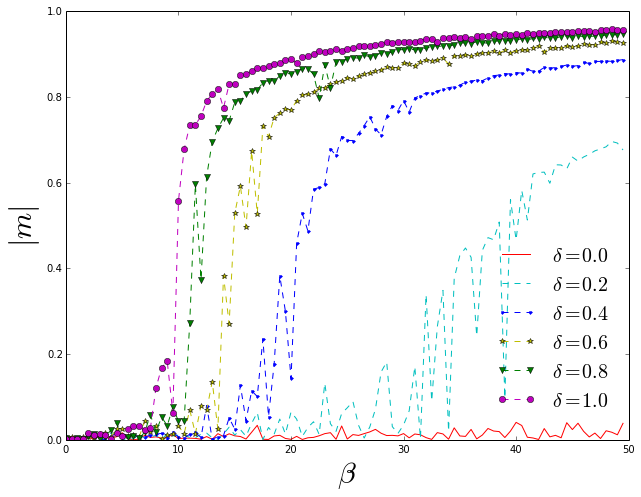
\includegraphics[width=1.0\textwidth]{mag-beta-delta.png}
  \caption{Gráfico da média das opiniões $m=\left<h\right>$ pela pressão social
      $\beta$ para diferentes valores do estilo cognitivo $\delta$}
    \label{m-b-d}
\end{figure}

A análise da figura mostra que o parâmetro $\delta$ possibilita o surgimento de
consenso na sociedade desde que seu valor seja diferente de zero e que haja
suficiente pressão social. Mais que isso, as curva de opinião são similares às
curvas de magnetização que caracterizam a transição de fases do modelo de Ising.
O diagrama de fases no espaço $\beta \times \delta$ é apresentado na figura
\ref{m-pd} 

\begin{figure}[h!]
  \centering
      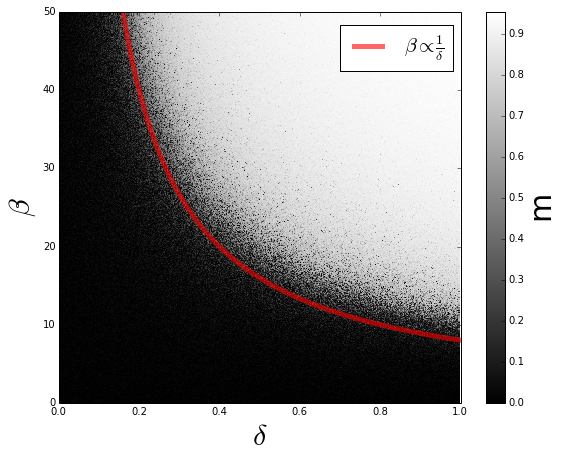
\includegraphics[width=1.0\textwidth]{mag-phase-diagram-greyscale.png}
  \caption{Gráfico do diagrama de fases de $m=\left<h\right>$ no espaço 
  $\beta \times \delta$}
  \label{m-pd}
\end{figure}

\subsubsection{Impedindo o consenso}

Como consequência do resultado para o consenso da sociedade, fica evidente que
esse modelo não suporta a manutenção de diferentes opiniões em situações de alta
pressão social. Em analogia com sistemas magnéticos, não é possível a
coexistência de regiões de diferentes magnetizações. Uma vez que tal coexistência
é interessante para avaliar a tolerância a
diferentes opiniões, uma forma de contornar essa limitação é necessária. 

A primeira tentativa nessa direção foi barrar o aprendizado no caso de extrema
discordância. Isso pode ser feito introduzindo um corte no potencial para
valores de concordância/discordância, $h_i h_j$, negativos e com grande módulo.
Se chamarmos o
ponto onde o corte é feito de $\tau$, o potencial de interação será

\[V_{\delta \tau}=-\frac{1+\delta}{2}h_ih_j+\frac{1-\delta}{2}|h_ih_j|+
              \frac{1}{2}(h_ih_j+\tau)-\frac{1}{2}|h_ih_j+\tau|
\]

Novamente, simulações de Monte Carlo foram feitas para analisar as curvas de
opinião e avaliar as condições em que há surgimento de consenso e os resultados
são apresentados na figura  \ref{m-b-t-3d}

% \begin{figure}[h!]
%   \centering
%       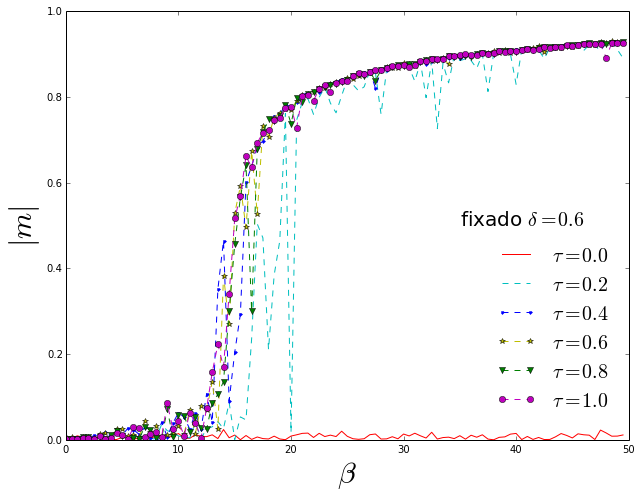
\includegraphics[width=1.0\textwidth]{mag-beta-tau.png}
%   \caption{Gráfico da média das opiniões $m=\left<h\right>$ pela pressão social
%       $\beta$ para diferentes valores para o ponto de corte $\tau$, para um
%   estilo cognitivo $\delta=0,6$ fixo.}
%     \label{m-b-t}
% \end{figure}

\begin{figure}[h!]
  \centering
      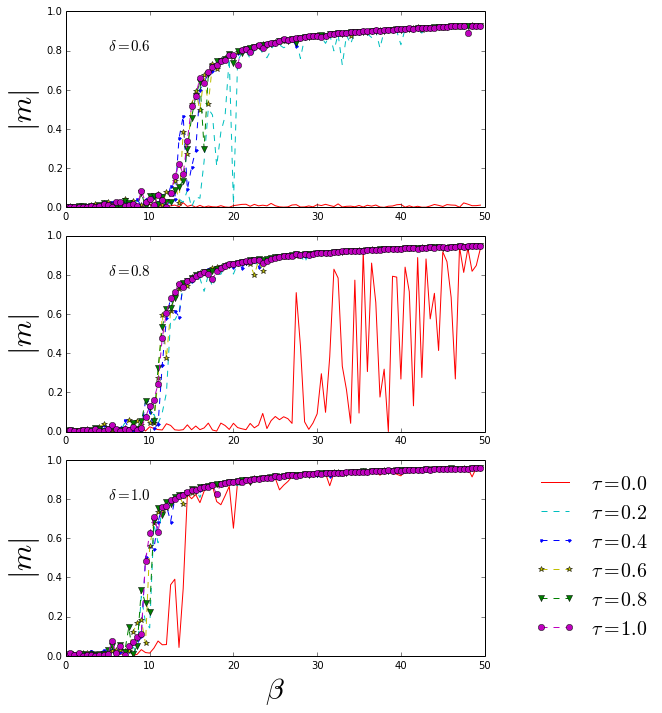
\includegraphics[width=1.0\textwidth]{mag-beta-tau-3-deltas.png}
  \caption{Gráfico da média das opiniões $m=\left<h\right>$ pela pressão social
      $\beta$ para diferentes valores para o ponto de corte $\tau$, para três
      valores do 
  estilo cognitivo $\delta=0.6$, $\delta=0.8$ e $\delta=1$}
    \label{m-b-t-3d}
\end{figure}

Note que o corte apenas dificulta do consenso, mas não impede seu
aparecimento execto quanto todo o aprendizado por discordância é eliminado
($\tau=0$).

\subsubsection{Busca de reputação}

Outra caraterística importante de instituições religiosas é a notoriedade e
influência dos
sacerdotes. Isso significa que um modelo adequado para entender esse fenêmeno
deve ser capaz de atribuir maior peso para a opiniões de indivíduos com morais
notoriedade.

Para atacar esse problema foi introduzida ao modelo uma dinâmica para as
relações entre indivíduos. Essa dinâmica possibilita que a interação entre dois
agentes seja fortalecida conforme eles concordem ou enfraquecida quando
discordam e que eles tenham um método de escolher com qual agente querem
interagir baseado na força da relação. Especificamente, foi atribuído um campo
$R_{ij}$ a cada aresta $(ij) \in E$ representando a reputação atribuída ao
agente $i$ pelo agente $j$. A probabilidade do agente $i$ ser escolhido pelo
agente $j$ para trocar informação em um dado momento depende de $R_{ij}$, que
cresce de acordo com a concordância entre os agentes cada vez que interagem.
Desse modo, era esperado que alguns agentes polarizassem as opiniões, adquirindo
grande reputação ao longo do história, o que seria refletido na relação entre
grau ("in-degree") médio e grau ("in-degree") máximo do grafo gerado pelas 
reputações. 

Os resultado das simulações de Monte Carlo com a dinâmica para a
reputação estão na figura \ref{R-b-d}

\begin{figure}[h!]
  \centering
      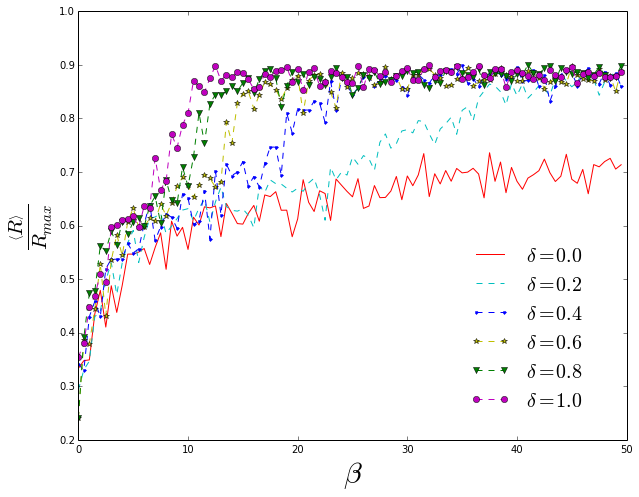
\includegraphics[width=1.0\textwidth]{R-beta-delta.png}
  \caption{Gráfico de $\frac{\left<R\right>}{R_{max}}$ pela pressão social
  $beta$ para diferentes valores do etilo cognitivo $\delta$}
  \label{R-b-d}
\end{figure}

\subsubsection{Sumário dos avanços obtidos}

Até então, foram estudados separadamente cada característica do fenômeno em foco,
além de algumas tentativas de uní-los num mesmo modelo. Embora a perspectiva
global ainda esteja fragmentada, nos próximos meses, espera-se, será possível
unir os resultados atuis numa compreensão mais concreta do fenômeno estudado.

Além da busca pela estruturação, alguns resultados recentes trazem possíveis
bases experimentais para o teste dos modelos \cite{Toorn} e
uma ampla base de dados pode fornercer diferentes perspectivas de
análise e, com sorte, dar suporte a previsões do modelo. \footnote{Uma base de
dados promissora é o atlas etnográfico de George P. Murdock, que pode ser
encontrado online em http://eclectic.ss.uci.edu/~drwhite/worldcul/atlas.htm}



\section{Cronograma de Atividades - 2014}

O resumo acima foi elaborado para justificar o cronograma para os próximos
meses. Com base nos resultados apresentados, é evidente que mais investigação é
necessária, não apenas no campo teórico como na comparação com dados
experimentais disponíveis. 

O cronograma proposto para os próximos meses é

\subsection{Primeiro Semestre de 2014}
\begin{itemize}
\item Abril e Maio: Obtenção de resultados e análise teórica e análise 
    estatística dos resultados das simulações e 
    tratamento analítico, com foco nas relações
    entre os resultados obtidos de modo a compor um modelo para fenômeno em
    estudo, a saber o comportamento típico de postura religiosa. Essa etapa
    requer estudo mais aprofundado dos resultados obtidos e a elaboração de
    alguns outros modelos para testar a conexão dos resultados obtidos até
    então.
    

\item Junho: Comparação com dados etnográficos e econômicos.

\item Julho: Eleboração da dissertação
\end{itemize}


\subsection{Segundo Semestre de 2014 (caso necessário)}
\begin{itemize}
\item Elaboração da dissertação
\item Defesa
\end{itemize}

\begin{thebibliography}{99}

\bibitem{Jaynes}E. T. Jaynes {\it Probability theory: The Logic of
    Science} Cambridge University Press, Cambridge (2003)

\bibitem{Ariel} A. Caticha Lecture Notes on information Theory,

\bibitem{mackay} MacKay D.J.C., \textit{Information Theory, Inference
    and Learning Algorithms}
Cambridge University Press, Cambridge, (2003).

\bibitem{Parisi} G. Parisi {\it et al, Spin Glasses and Beyond}

\bibitem{Engel} A. Engel and C. van den Broeck {\it Statistical
    Mechanics of Learning}

\bibitem{Nishimori} Nishimori, Statistical Physics of Spin Glasses and Information Processing: An Introduction

\bibitem{Ostrom}Ostrom, Elinor (1990). Governing the Commons: The Evolution of Institutions for Collective Action. Cambridge University Press. ISBN 0-521-40599-8; Ostrom, Elinor (July 2009). "A General Framework for Analyzing Sustainability of Social-Ecological Systems". Science 325: 419–422.

\bibitem{Hardin}Garrett Hardin
"The Tragedy of the Commons". Science 162 (3859): 1243–1248. 1968.

\bibitem{Strandburg}Michael J. Madison, Brett M. Frischmann
and Katherine J. Strandburg, 
Legal Studies Research Paper Series
Working Paper No. 2008-26
August 2008

\bibitem{Estes}William K. Estes, Research and Theory on the
Learning of Probabilities,
Journal of the American Statistical Association, Vol. 67, No. 337
(Mar., 1972), pp. 81-102

\bibitem{CaVi}N.Caticha and R.Vicente ¨Agent-based social psycology: from neurocognitive processes to social data¨ Volume: 14, Issue: 5(2011) pp.711-731 Advances in Complex Systems (ACS)

\bibitem{Settle2010a}Settle, Jaime E Dawes, Christofer T Christakis, Nicholas A Fowler, James H (2010) 72,4 1189 ¨Friendships Moderates an Association Between a Dopamine Gene and Political Ideology.¨ The journal of politicsz

\bibitem{Kandel} Kandel, et al, Essentials of neural sciences and behavior.


\bibitem{Dunbar} R. Dunbar,  Grooming, Gossip, and the
Evolution of Language. Faber, London (1997)

\bibitem{Eisenberger} Eisenberger, N., Lieberman, M., and Williams, K., Does rejection hurt? An fMRI
study of social exclusion, Science 302 (2003) 290-292.

\bibitem{Mazur} Allan Mazur,
Biosociology
of Dominance
and Deference
ROWMAN and LITTLEFIELD PUBLISHERS, INC.
(2005

 \bibitem{Pumain}
Hierarchy in Natural
and Social Sciences
edited by
Denise Pumain, Springer (2006)

\bibitem{Bohem}Christopher Boehm
Hierarchy in the Forest
The Evolution of
Egalitarian Behavior, Harvard University Press (2001)

\bibitem{Earle} Timothy Earle,
How Chiefs came to power, Stanford University Press (1997)

\bibitem{Salzman} Philip Carl Salzman, Pastoralists: Equality, Hierarchy and
the State. Westview Press (2004)

\bibitem{Fleagle}Edited by
John G. Fleagle
Charles H. Janson
Kaye E. Reed, Primate Communities
Cambridge University Press (2004)

\bibitem{Wason} Paul K. Wason, The archaeology of rank
Cambridge University Press (1994)

\bibitem{Sassaman} Kenneth E. Sassaman, Journal of Archaeological Research Vol 12 september 2004

\bibitem{Menger} Carl Menger
On the Origins of Money
Economic Journal, volume 2,(1892) p. 239-55.
translated by C.A. Foley

\bibitem{Maisels}Charles Keith Maisels, The Emergence of
Civilization:
From hunting and gathering to
agriculture, cities, and the state in the
Near East,
Routledge   (2005)

\bibitem{CatichaetalA} N. Caticha, R. Calsaverini, R. Vicente, {\it
Cognitive limits and Breakdown of the Egalitarian Society} preprint   (2012)

\bibitem{Schonmannetal2011a} R. Schonmann, R. Vicente e N. Caticha
Two-level Fisher-Wright framework with selection and migration: An approach to studying evolution in group structured populations.
arXiv:1106.4783 (2011)

\bibitem{Perreault}C. Perreault, C. Moya, and R. Boyd. A Baysian approach to the evolution of social learning. Evolution and Human Behavior, Proofs posted online April 2012

\bibitem{Jonatas}
Jônatas Eduardo da Silva César. Mecânica Estatística de Sistemas de Agentes
Baysianos: Aplicação à Teoria dos Fundamentos Morais. Tese defendida em 2014

\bibitem{visujeca} R. Vicente, A. Susemihl, J.P. Jericó, N. Caticha. Moral
    foundations in an interacting neural networks society

\bibitem{Toorn}Jojanneke van der Toorn, Jaime L. Napier and John F. Dovidio. We the People: Intergroup Interdependence Breeds Liberalism
Social Psychological and Personality Science published online 5 December 2013

\bibitem{Haidt} Graham, Jesse; Haidt, Jonathan; Nosek, Brian A.
    Liberals and conservatives rely on different sets of moral foundations.
Journal of Personality and Social Psychology, Vol 96(5), May 2009, 1029-1046

\end{thebibliography}    

\end{document}


